% Section fragment: requires Chinese support, amsmath, graphicx and booktabs.
\subsection{考虑尺寸收缩的烘干过程模型}
\subsubsection{移动边界与模型假设}

将药材视为轴对称长圆柱，忽略轴向传递及长度变化。半径 $R(t)$ 由实测序列线性插值获得，
令 $\xi=r/R(t)$。在仿射收缩假设下，材料点的 $\xi$ 不变。
局部含水率为 $C$，温度 $T$ 以摄氏度表示，物性为
\begin{align}
\rho_{\mathrm{eff}}(C)&=760+90C,&
c_p(C)&=1850+\frac{2150C}{1+C},\\
k(C)&=0.12+\frac{0.20C}{1+C},&
D(C,T)&=4.2\times10^{-4}\exp\left(-\frac{0.30}{C}-\frac{3850}{T+273.15}\right).
\end{align}
初始条件为 $T=28\,^\circ\mathrm C$、$C=2.55$、$R_0=0.02\,\mathrm m$。
不含潜热基准方程及边界条件为
\begin{align}
C_t&=\frac{1}{R^2\xi}\frac{\partial}{\partial\xi}(\xi D C_\xi),\\
\rho_{\mathrm{eff}}c_pT_t&=\frac{1}{R^2\xi}\frac{\partial}{\partial\xi}(\xi k T_\xi),\\
C_\xi(0,t)&=T_\xi(0,t)=0,\\
-\frac{D}{R}C_\xi(1,t)&=h_m(C_s-C_a),\\
-\frac{k}{R}T_\xi(1,t)&=h(T_s-T_a).
\end{align}
其中 $h=25\,\mathrm{W/(m^2\,K)}$，$h_m=8.0\times10^{-7}\,\mathrm{m/s}$。
收缩同时改变内部传递尺度、边界条件和固定距离采样位置，不能仅归结为 $R^{-2}$ 放大。
主方案在 $4\,\mathrm h$ 后维持实测末值 $50.165\,^\circ\mathrm C$ 和 $0.04986$；
另一方案取 $50\,^\circ\mathrm C$，湿度仍维持末值。

\subsubsection{潜热对照与闭合限制}

取固定参数 $L_v=2.383\times10^6\,\mathrm{J/kg}$，令
\begin{align}
\rho_{d0}&=\frac{760+90C_0}{1+C_0},&
\rho_d(t)&=\rho_{d0}\left(\frac{R_0}{R(t)}\right)^2,\\
J_w&=\rho_dh_m(C_s-C_a).
\end{align}
表面蒸发模型将热边界改为
\begin{equation}
-\frac{k}{R}T_\xi(1,t)=h(T_s-T_a)+L_vJ_w.
\end{equation}
体积型替代模型保留原热边界，在热方程右侧加入 $L_v\rho_d C_t$。
两项不同时使用，以免重复计入潜热。体积处理将局部含水率变化作为相变耗能代理，
不代表内部蒸发机制已验证。
仿射收缩干密度与经验有效密度采用不同闭合，缺少独立数据证明局部总质量关系完全一致。
亦无证据证明潜热已被经验参数吸收，不含潜热仅作为明确的基准假设。

\subsubsection{数值求解与结果}

采用表面加密有限体积法、三点 Gauss 界面物性平均和 BDF 时间积分，相对容差为 $10^{-11}$。
连续临界时间和整分钟输出时间分别为
\begin{align}
t_*&=\inf\{t:\max_r C(r,t)<0.15\},\\
t_{60}&=\min\{60k:\max_r C(r,60k)<0.15,\ k\in\mathbb N\}.
\end{align}
对本次连续向下穿越阈值的解，根满足 $\max_r C(r,t_*)=0.15$。
在根后继续积分至下一整分钟，并用未舍入值检查严格不等式。

\begin{table}[htbp]
\centering
\caption{不同环境外推下的烘干时间及终点半径}
\label{tab:a4_times}
\begin{tabular}{lrrr}
\toprule
环境外推 & $t_*/\mathrm h$ & $t_{60}/\mathrm h$ & $R(t_{60})/\mathrm{cm}$\\
\midrule
数据末值 & 50.8243 & 50.8333 & 1.2000\\
$50\,^\circ\mathrm C$、湿度末值 & 51.0875 & 51.1000 & 1.2000\\
\bottomrule
\end{tabular}
\end{table}

800 单元结果见表~\ref{tab:a4_times}。
$72\,\mathrm h$ 观测末值 $1.198\,\mathrm{cm}$ 并非上述烘干终点半径。
末值方案末行中心含水率约为 $0.14998317$，显示为 $0.1500$ 是舍入所致。

\begin{figure}[htbp]
\centering
\IfFileExists{../04-pic/fig01_drying.png}
{\includegraphics[width=.96\linewidth]{../04-pic/fig01_drying.png}}
{\includegraphics[width=.96\linewidth]{04-pic/fig01_drying.png}}
\caption{末值环境方案的水分浓度及半径变化}
\label{fig:a4_drying}
\end{figure}

\begin{table}[htbp]
\centering
\caption{不含潜热基准模型的水分浓度}
\label{tab:a4_field}
\begin{tabular}{rrrrr}
\toprule
时间$/\mathrm h$ & 中心 & $0.5\,\mathrm{cm}$ & $1.0\,\mathrm{cm}$ & 表面\\
\midrule
6 & 1.7172 & 1.5357 & 1.0217 & 0.4217\\
12 & 0.7343 & 0.6518 & 0.4069 & 0.1667\\
18 & 0.4066 & 0.3668 & 0.2388 & 0.0889\\
24 & 0.2837 & 0.2599 & 0.1783 & 0.0671\\
30 & 0.2253 & 0.2085 & 0.1488 & 0.0593\\
36 & 0.1921 & 0.1790 & 0.1312 & 0.0558\\
42 & 0.1706 & 0.1598 & 0.1196 & 0.0539\\
48 & 0.1556 & 0.1463 & 0.1113 & 0.0529\\
50.8333 & 0.1500 & 0.1412 & 0.1081 & 0.0525\\
\bottomrule
\end{tabular}
\end{table}

\subsubsection{收敛、敏感性与模型局限}

1600 单元结果为 $50.8242226\,\mathrm h$，与 800 单元相差约 $0.216\,\mathrm s$。
四位小数仍可能变化，不能认定末位已收敛。
七种环境外推在同一 400 单元网格下为 $50.824522$--$51.138994\,\mathrm h$，
相对末值方案最大增加约 $0.619\%$。
同为末值环境和 400 单元，不含潜热、表面潜热及体积潜热临界时间分别为
$50.824522$、$56.164294$、$58.253124\,\mathrm h$，潜热假设不可不加讨论地忽略。

第三组物性固定半径模型与本模型同时改变物性及几何，约 $11.1\%$ 时间差不能称为收缩净效应。
保持第四组物性的 400 单元控制试验中，固定 $2\,\mathrm{cm}$ 半径为
$129.093760\,\mathrm h$，观测收缩半径为 $50.824522\,\mathrm h$，条件性变化约为 $-60.630\%$。
该结果仅为指定模型的反事实对照，不是实验因果测量。
离散恒等式及积分残差只验证实现一致性，不等同于完整物理守恒证明。
环境外推、密度闭合、相变位置及经验参数仍需独立验证。
